% Sherlockii je t'aime <3 - Clément Geiger et Raphaël Lizé

\documentclass[twoside]{article}
\usepackage{hyperref}


\usepackage{graphicx}
\usepackage{subfig}
\usepackage{placeins}


% Language settings:
\usepackage[francais]{babel}
\usepackage[utf8]{inputenc}

\usepackage[T1]{fontenc}


% Font settings:
\usepackage{charter}


\title{Sherlockii je t'aime <3}
\author{Clément Geiger et Raphaël Lizé}
% Page layout settings
\usepackage{geometry}
\geometry{
	a4paper,  % 21 x 29,7 cm
	body={150mm,230mm},
	left=30mm, 
	top=30mm,
	headheight=7mm, 
	headsep=4mm,
	marginparsep=4mm,
	marginparwidth=27mm
}


% Spacing:
\usepackage{setspace}


% Headers and footers:
\usepackage{fancyhdr}
\pagestyle{fancy}
          \fancyhf{}
          \fancyfoot[LE,RO]{\thepage}
          % Rulers width
          \renewcommand{\footrulewidth}{.3pt}
          \renewcommand{\headrulewidth}{.3pt}
\fancyhead[RO,RE]{Clément Geiger et Raphaël Lizé}
\fancyfoot[LO,RE]{Sherlockii je t'aime <3}


% Vars & functs
\newcommand\PIXPATH{./docs/pics}
\renewcommand{\labelitemi}{$\diamond$}


% Begining of the document
\begin{document}
\large
\onehalfspacing

	%Including all the files:

% Fichier 0.premiere_page.tex

% Page de garde
% Title:
\maketitle

\thispagestyle{empty}

\vfill

\begin{center}

\includegraphics[scale=0.50]{\PIXPATH/insa.jpg}
\end{center}

\pagebreak

% Fichier 1.diag.tex

\section*{Introduction}
Il s'agit de créer un «meta» système expert chargé
d'évaluer le premier et de l'améliorer.

%\vfill

\section{Modèle de maintenance automatique.}
\begin{figure}[!h]
\begin{center}
        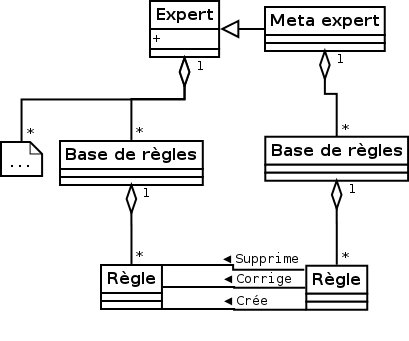
\includegraphics[scale=0.7]{\PIXPATH/diag}
        \caption{Modèle de maintenance automatique.}
\end{center}
\end{figure}

% Fichier 2.maintenance.tex

\section{Maintenance évolutive}

L'intérêt d'un système expert est proportionnel à sa capacité à répondre
de manière exacte à tous les problèmes du domaine de son expertise. Il 
s'agit donc de s'assurer qu'il évolue de façon à pouvoir traiter des
problèmes nouveaux, qui n'ont pas été prévus lors de sa conception.

La maintenance évolutive, dans cette optique, va permettre d'ajouter (ou
de supprimer) des règles, bases de règles... et tout autre élément entrant
dans le raisonnement.

L'intérêt, d'une telle maintenance est d'alonger la durée de vie du
logiciel, évitant ainsi des dépenses en temps et en argent pour 
développer un système similaire mais contenant plus de règles.

Idéalement, une telle maintenance serait automatique: un logiciel serait
capable de se mettre à jour tout seul, avac pour seule intervention
humaine la répartition des torts d'une situation que le système n'arrive
pas à départager. 

% The end
\end{document}

